\section{Zielsetzung}
\label{sec:Zielsetzung}
Es soll die Quantennatur der Elektronenhülle von Atomen gezeigt werden. Weiterhin soll ein Zusammenhang zwischen
der Anregungsenergie und der Wellenlänge des emittierten Lichts hergestellt werden. Mit den daruas erhaltenen
Erkentnissen lassen sich die Bohrschen Postulate teilweise bestätigen. Außerdem wird die Energieverteilung der
Elektronen bestimmt.

\section{Theorie}
\label{sec:Theorie}
Es wird Hg-Dampf mit passender Dichte mit möglichst monoenergetischen Elektronen beschossen. Dabei treten
elastische und unelastische Stöße auf. Aus der Energiedifferenz der Elektronen vor und nach dem Stoß lässt
sich dann die vom Hg-Atom aufgenommene Energie bestimmen. Die unelastischen Stöße werden dabei verwendet, um
die Atome aus dem Grundzustand $E_{\symup{0}}$ in den ersten angeregten Zustand $E_{\symup{1}}$ zu heben.
Für die Energiedifferenz gilt dann
\begin{equation}
    \label{eqn:Ediff}
    \frac{m_{\symup{0}}v_{\symup{vor}}^2}{2} - \frac{m_{\symup{0}}v_{\symup{nach}}^2}{2}
    = E_{\symup{1}} - E_{\symup{0}}\,.
\end{equation}
Die Energien lassen sich mit der Gegenfeldmethode bestimmen.

\subsection{Aufbau und Ablauf}
\label{sec:AufbauAblauf}
In einem evakuierten Gefäß ist ein Tropfen Quecksilber, der nach der Dampfdruckkurve verdampft. Dadurch
hängt der Gleichgewichtsdampfdruck $p_{\symup{sät}}$ von der Temperatur $T$ ab. Im Gefäß wird ein Draht aus einem
hochschmelzenden Metall, wie z.B. Wolfram, mittels Gleichstrom auf Rotglut erhitzt, so dass durch den
glühelektrischen Effekt Elektronen frei werden, die sich wie eine Wolke um den Draht legen. Dieser Effekt wird
durch ein Oxid eines Erdalkalimetalls, das auf den Draht gestrichen wurde und eine geringere Austrittsarbeit
$W$ als der Draht hat, so dass mehr Elektronen frei werden. Um die Elektronen zu beschleunigen, wird eine
netzförmige Elektrode gegenüber zum Draht angebracht, an der eine Gleichspannung $U_{\symup{B}}$ zur Beschleunigung
angelegt wird. Eine schematische Darstellung des Versuchaufbaus ist in \autoref{fig:Aufbau} zu sehen.
\begin{figure}
    \centering
    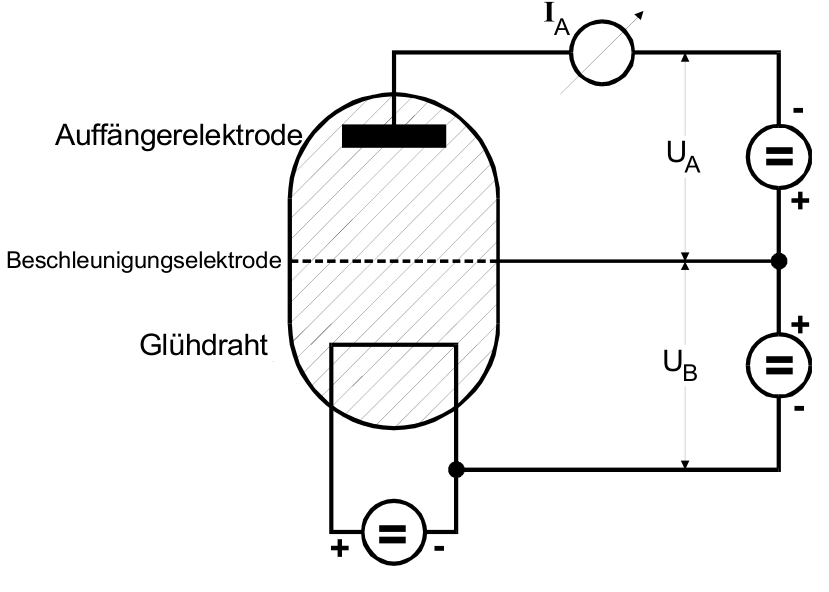
\includegraphics[width=0.7\textwidth]{Bilder/SchematischerAufbau.png}
    \caption{Schematischer Aufbau der Franck-Hertz Apparatur \cite{sample}.}
    \label{fig:Aufbau}
\end{figure}
Nach der Beschleunigungsstrecke haben die Elektronen die Energie
\begin{equation}
    \label{eqn:E_Beschleunigung}
    \frac{m_{\symup{0}} v_{\symup{vor}}^2}{2} = \symup{e}_{\symup{0}} U_{\symup{B}}
\end{equation}
solange sie vor der Beschleunigung die Geschwindigkeit 0 hatten. Hinter der Beschleunigungselektrode befindet
sich eine Auffängerelektrode an der mit einem geeigneten Messgerät der Auffängerstrom $I_{\symup{A}}$ messbar ist.
Da die Auffängerelektrode eine geringere Spannung $U_{\symup{A}}$ als die Beschleunigungselektrode hat, müssen die
Elektronen, damit sie an der Auffängerelektrode ankommen, die Ungleichung
\begin{equation}
    \label{eqn:E_Ungleichung}
    \frac{m_{\symup{0}}}{2} v_{\symup{z}}^2 \geq \symup{e}_{\symup{0}} U_{\symup{A}}
\end{equation}
erfüllen. Im Beschleunigungsraum befinden sich nun die Hg-Atome, so dass die Elektronen mit ihnen zusammenstoßen.
Bei geringer Elektronenenergie treten nur elastische Stöße auf. Da das Massenverhältnis von Elektron und Hg-Atom
etwa $\frac{1}{1836 \cdot 201}$ beträgt, ergibt sich eine relativ geringe Energieabgabe von
\begin{equation}
    \label{eqn:EnergieAbgabe}
    \Delta E = \frac{4 m_{\symup{0}} M}{(m_{\symup{0}} + M)^2} E \approx 1,1\cdot 10^{-5} E\,.
\end{equation}
Die dabei vollzogenen Richtungsänderungen können dabei aber beträchtlich sein. Haben die Elektronen mindestens die
Energiedifferenz, die es braucht ein Hg-Atom aus dem Grundzustand in den ersten angeregten Zustand zu bringen,
stoßen sie nicht mehr elastisch sondern unelastisch. Dabei behalten sie die Energie $E - (E_{\symup{1}} - 
E_{\symup{0}})$, d.h. sie geben nur die Energie ab, um ein Hg-Atom anzuregen. Das emittierte Lichtquant hat dann
die Energie
\begin{equation}
    \label{eqn:Emission}
    h\nu = E_{\symup{1}} - E_{\symup{0}}\,.
\end{equation}
Dabei ist $h$ das Plancksche Wirkungsquantum und $\nu$ die Frequenz des Lichtquants.
Um die Anregung der Hg-Atome zu beobachten, wird nun der Auffängerstrom $I_{\symup{A}}$ in Abhängigkeit der
Beschleunigungsspannung gemessen. Erreichen die Elektronen die Energie $E_{\symup{1}} - E_{\symup{0}}$ geben
sie ihre Energie an die Hg-Atome ab und haben anschließend fast keine Energie mehr, so dass der Auffängerstrom
auf Null fällt. Wird die Beschleunigungsspannung weiter erhöht so können mehrer Peaks entstehen. Eine schmematische
Darstellung der idealisierten Kurve ist in \autoref{fig:Kurveideal} zu sehen. Der Abstand der Maxima ergibt sich
dann zu
\begin{equation}
    \label{eqn:Spannung}
    U_{\symup{1}} = \frac{1}{\symup{e}_{\symup{0}}}\left(E_{\symup{1}}-E_{\symup{0}}\right).
\end{equation}
\begin{figure}
    \centering
    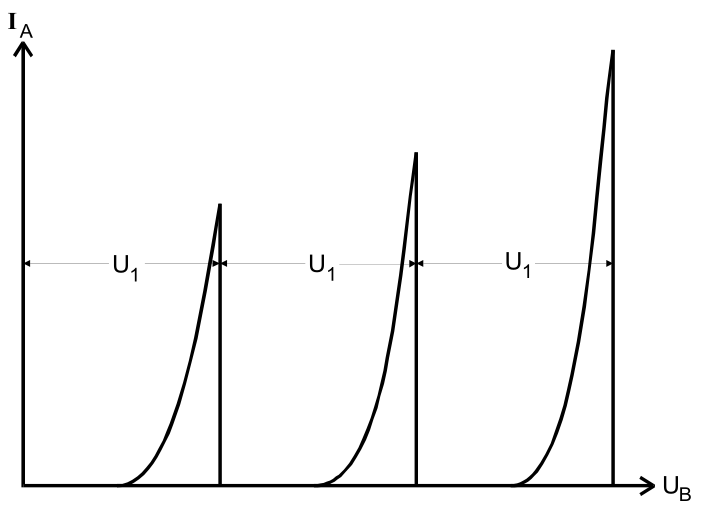
\includegraphics[width=0.7\textwidth]{Bilder/idealisierteKurve.png}
    \caption{Idealisierte Kurve des Auffängerstroms in Abhängigkeit der Beschleunigungsspannung \cite{sample}.}
    \label{fig:Kurveideal}
\end{figure}

\subsection{Einflüsse auf die Gestalt der Franck-Hertz Kurve}
\label{sec:Einflüsse}
Die gemessene Kurve unterscheidet sich teilweise signifikant von der theoretisch bestimmten, so dass Nebeneffekt
in bei der Theoriekurve berücksichtigt werden müssen.

\subsubsection{Kontaktpotential}
\label{Kontaktpotential}
Das Beschleunigungspotential zwischen Glühdraht und Beschleunigungselektrode ist aufgrund der unterschiedlichen
verwendeten Materialien und deren Austrittsarbeiten verschieden.
\begin{figure}
    \centering
    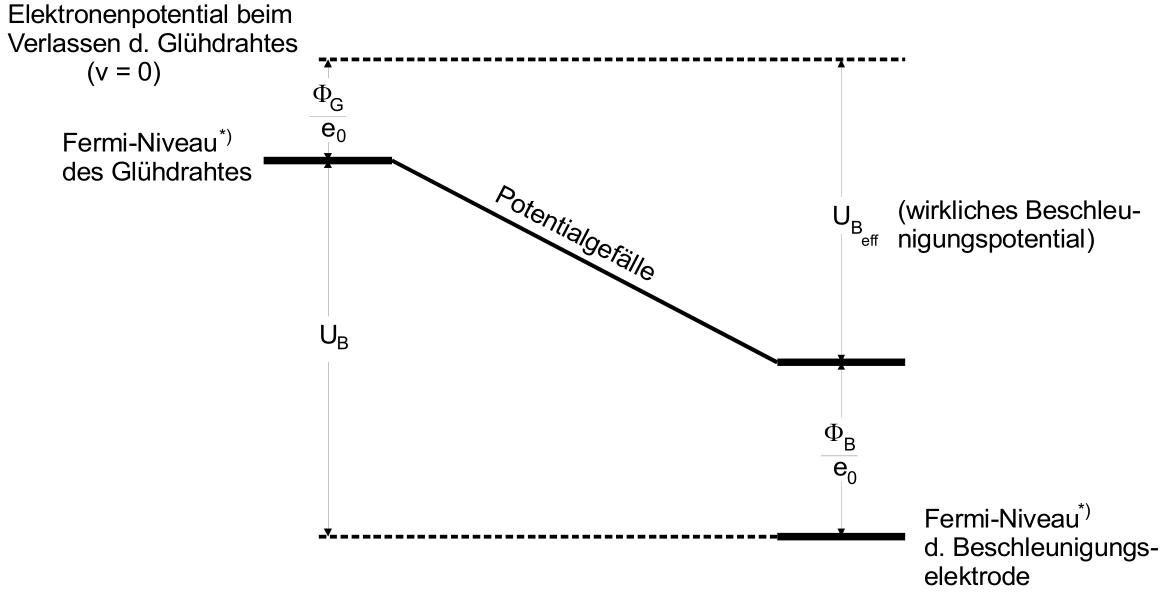
\includegraphics[width=0.7\textwidth]{Bilder/Kontaktpotential.png}
    \caption{Darstellung des Kontaktpotentials \cite{sample}.}
    \label{fig:Kontaktpotential}
\end{figure}
Die effektive Beschleunigungsspannung kann dann aus dem Potentialgefälle zu
\begin{equation}
    \label{eqn:Ueff}
    U_{\symup{eff}} = U_{\symup{B}} - \frac{1}{\symup{e}_{\symup{0}}}\left(\Phi_{\symup{B}}-\Phi_{\symup{G}}\right)
\end{equation}
bestimmt werden. Wobei $K$ als Kontaktpotential definiert durch
\begin{equation}
    \label{eqn:Kontaktpotential}
    K = \frac{1}{\symup{e}_{\symup{0}}}\left(\Phi_{\symup{B}}-\Phi_{\symup{G}}\right)
\end{equation}
definiert wird.

\subsection{Einfluss durch die Energieverteilung der Elektronen}
\label{sec:Energieverteilung}
Die durch den glühelektrischen Effekt losgelösten Elektronen haben unterschiedliche Anfangsgeschwindigkeiten,
die der Fermi-Dirac-Statistik gehorchen, so dass dadurch die Kurve so bald sie sich einem Maximum annähert,
immer geringer steigt. Weiterhin sorgt dieser Effekt dafür, dass anstatt eines abrupten Abfalls auf 0 Minima
in der Frank-Hertz Kurve zu beobachten sind.

\subsection{Dampfdruckkurve}
\label{sec:Dampfdruckkurve}
Damit die für das Experiment benötigten Zusammenstöße vorkommen, muss die freie Weglänge $\bar{w}$ für
eine hohe Trefferwahrscheinlichkeit kleiner als der Abstand $a$ zwischen der Kathode und der Beschleunigungskathode
sein. Nach der kinetischen Gastheorie bestimmt sich $\bar{w}$ in Abhängigkeit des Sättigungsdampfdrucks
$p_{\symup{sät}}$ zu
\begin{equation}
    \label{eqn:w}
    \bar{w} = \frac{0,0029}{p_{\symup{saet}}}.
\end{equation}
Dabei wird $\bar{w}$ in $\unit{\centi\meter}$ und $p_{\symup{saet}}$ in $\unit{\milli\bar}$ angegeben.
Der Sättigungsdampfdruck ergbit sich aus der Dampfdruckkurve durch
\begin{equation}
    \label{eqn:Dampfdruck}
    p_{\symup{saet}}(T) = 5,5\cdot e^{\frac{-6876}{T}}.
\end{equation}
Dabei ist $p$ wieder in $\unit{\milli\bar}$ und $T$ in $\unit{\kelvin}$ angegeben. Insgesamt muss $\bar{w}$
$1000$ bis $4000$ mal kleiner als $a$ sein, damit die Apparatur otpimal arbeitet.

\subsection{Aufbau der Hg-Elektronenhülle}
\label{sec:Elektronenhülle}
Der Grundzustand des Hg-Atoms $n=6$, $S=0$ und $L=0$ besitzt keine Feinstruktur und befindet sich im so genannten
Singulett-System. Der angeregte Zustand ist dann nicht $n=7$, $S=0$ und $L=0$, sondern er geht durch die
Spin-Bahn-Kopplung in eins der in \autoref{fig:Termschema} gezeigten Triplett-Systeme über.
\begin{figure}
    \centering
    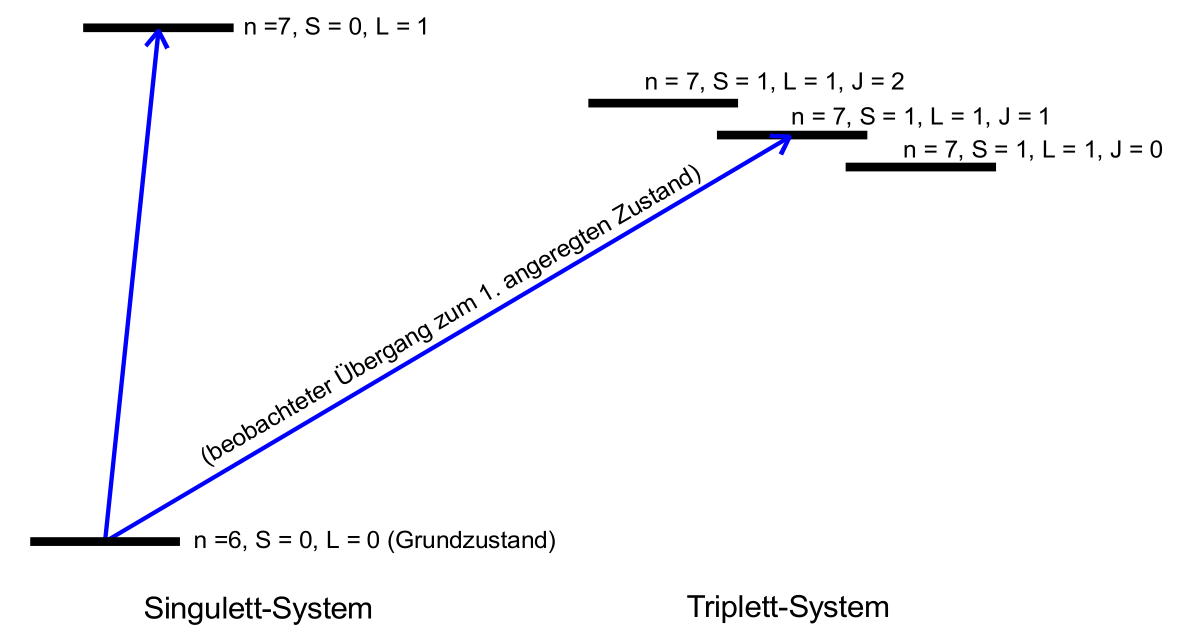
\includegraphics[width=0.7\textwidth]{Bilder/Termschema.png}
    \caption{Termschema des Hg-Atoms \cite{sample}.}
    \label{fig:Termschema}
\end{figure}